\chapter{Supplementary Figures}
\label{Chap:E}
\pagestyle{headings}

\section{Supplementary figures for study in Chapter 3}
\begin{sidewaysfigure}
    \centering
    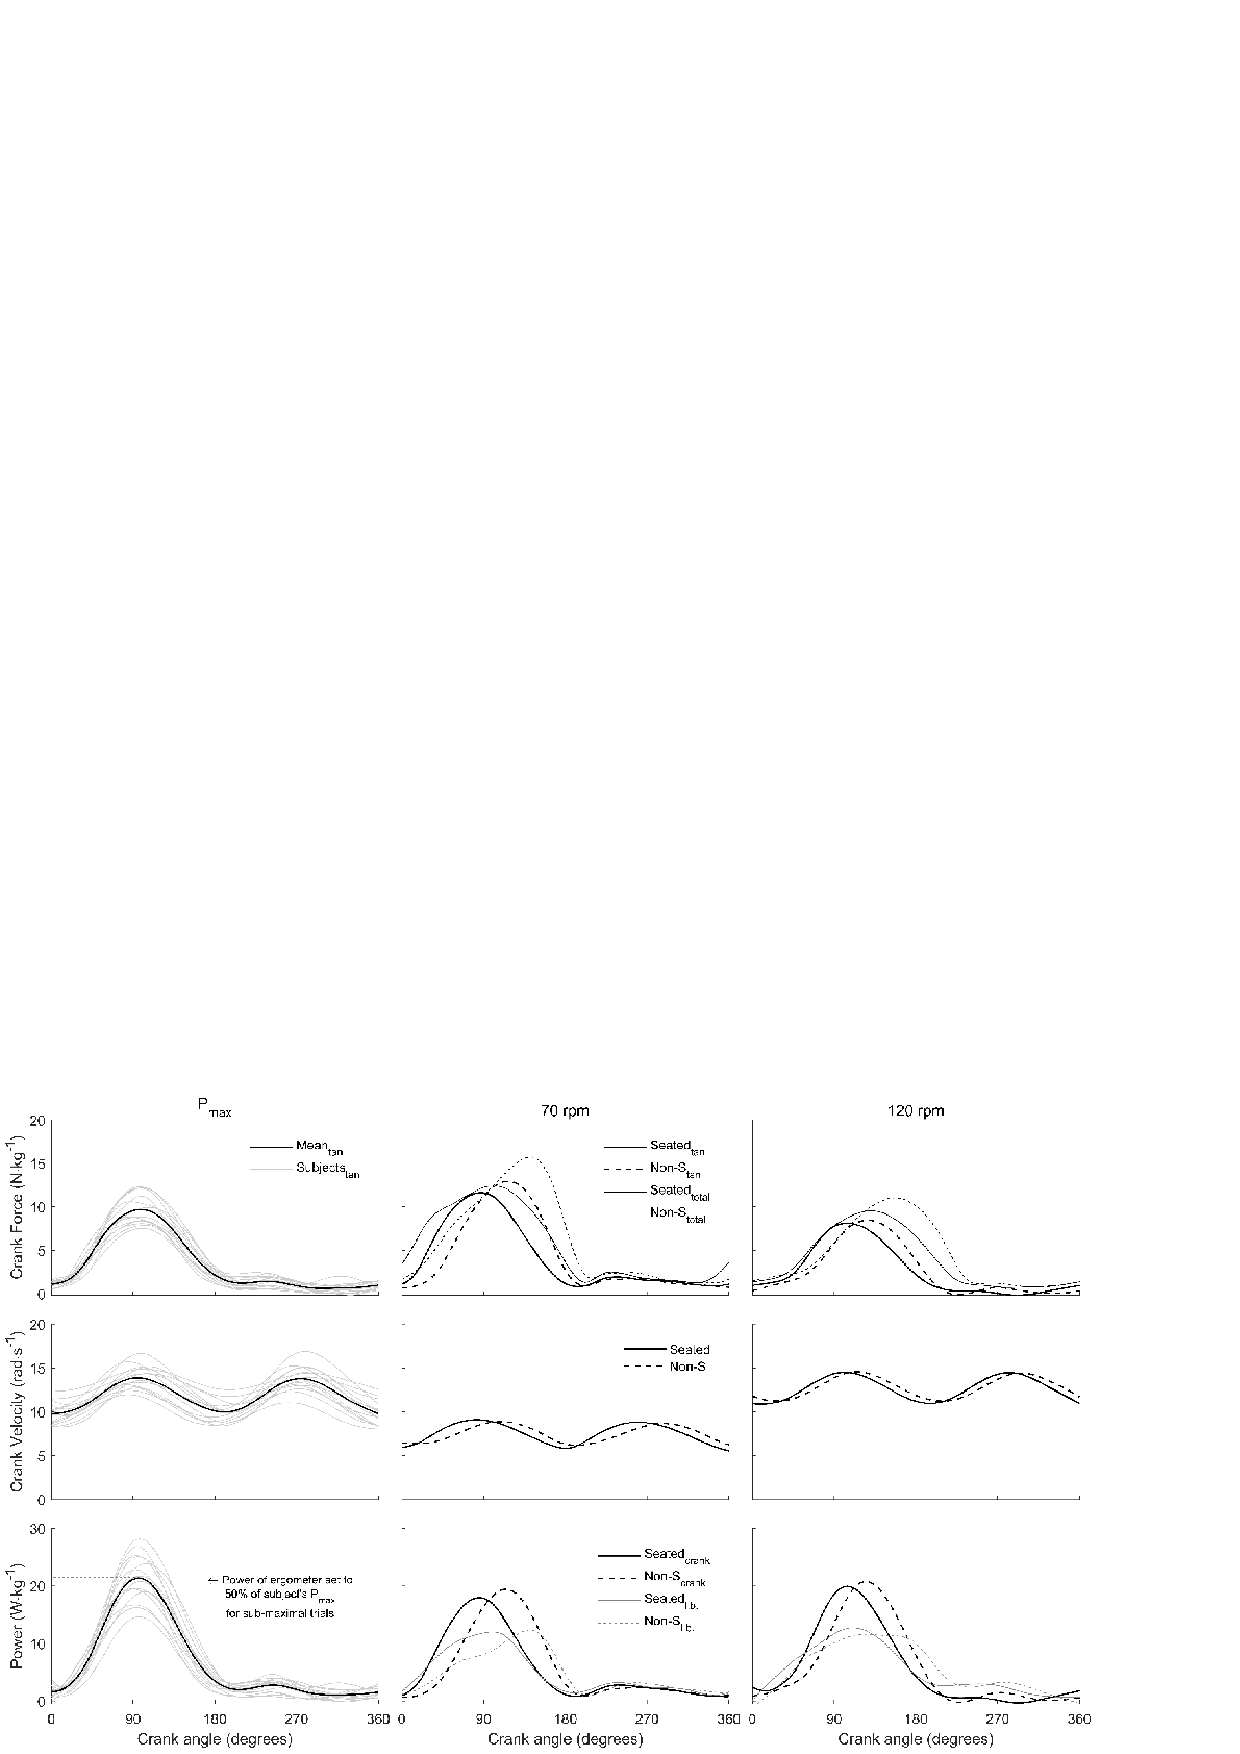
\includegraphics[width=0.9\textwidth]{SupplementaryFigures/Study1_supp1.png}
    \caption[Peak crank power far exceeds peak power generated by the leg during seated and non-seated cycling, suggesting that additional power is generated by muscles in the upper body or or the rider's CoM.]{\textbf{Peak crank power far exceeds peak power generated by the leg during seated and non-seated cycling, suggesting that additional power is generated by muscles in the upper body or or the rider's CoM.} Participant and group mean crank force, velocity and power during the P$_{max.i}$ trials (left column) as well as a comparison of crank and leg power during the sub-maximal trials at 70 rpm (centre) and 120 rpm (right).}
    \label{fig:m1sdc1}
\end{sidewaysfigure}

\begin{table}
    \centering
    \includegraphics[width=0.9\textwidth]{SupplementaryFigures/Study1_supp2.png}
    \caption[Peak knee extension moments decreased, while range of motion at the knee increased when non-seated at 70 rpm compared to when seated.]{\textbf{Peak knee extension moments decreased, while range of motion at the knee increased when non-seated at 70 rpm compared to when seated.} Group mean ($\pm$SD) peak angle (\textdegree), velocity (\textdegree s$^{-1}$) and joint moments (Nm$\cdot$kg$^{-1}$) at the hip, knee, and ankle during high power output cycling (10.74 W$\cdot$kg$^{-1}$) at low (70 rpm) and high (120 rpm) cadence.}
    \label{tab:m1sdc2}
\end{table}

\begin{figure}
    \centering
    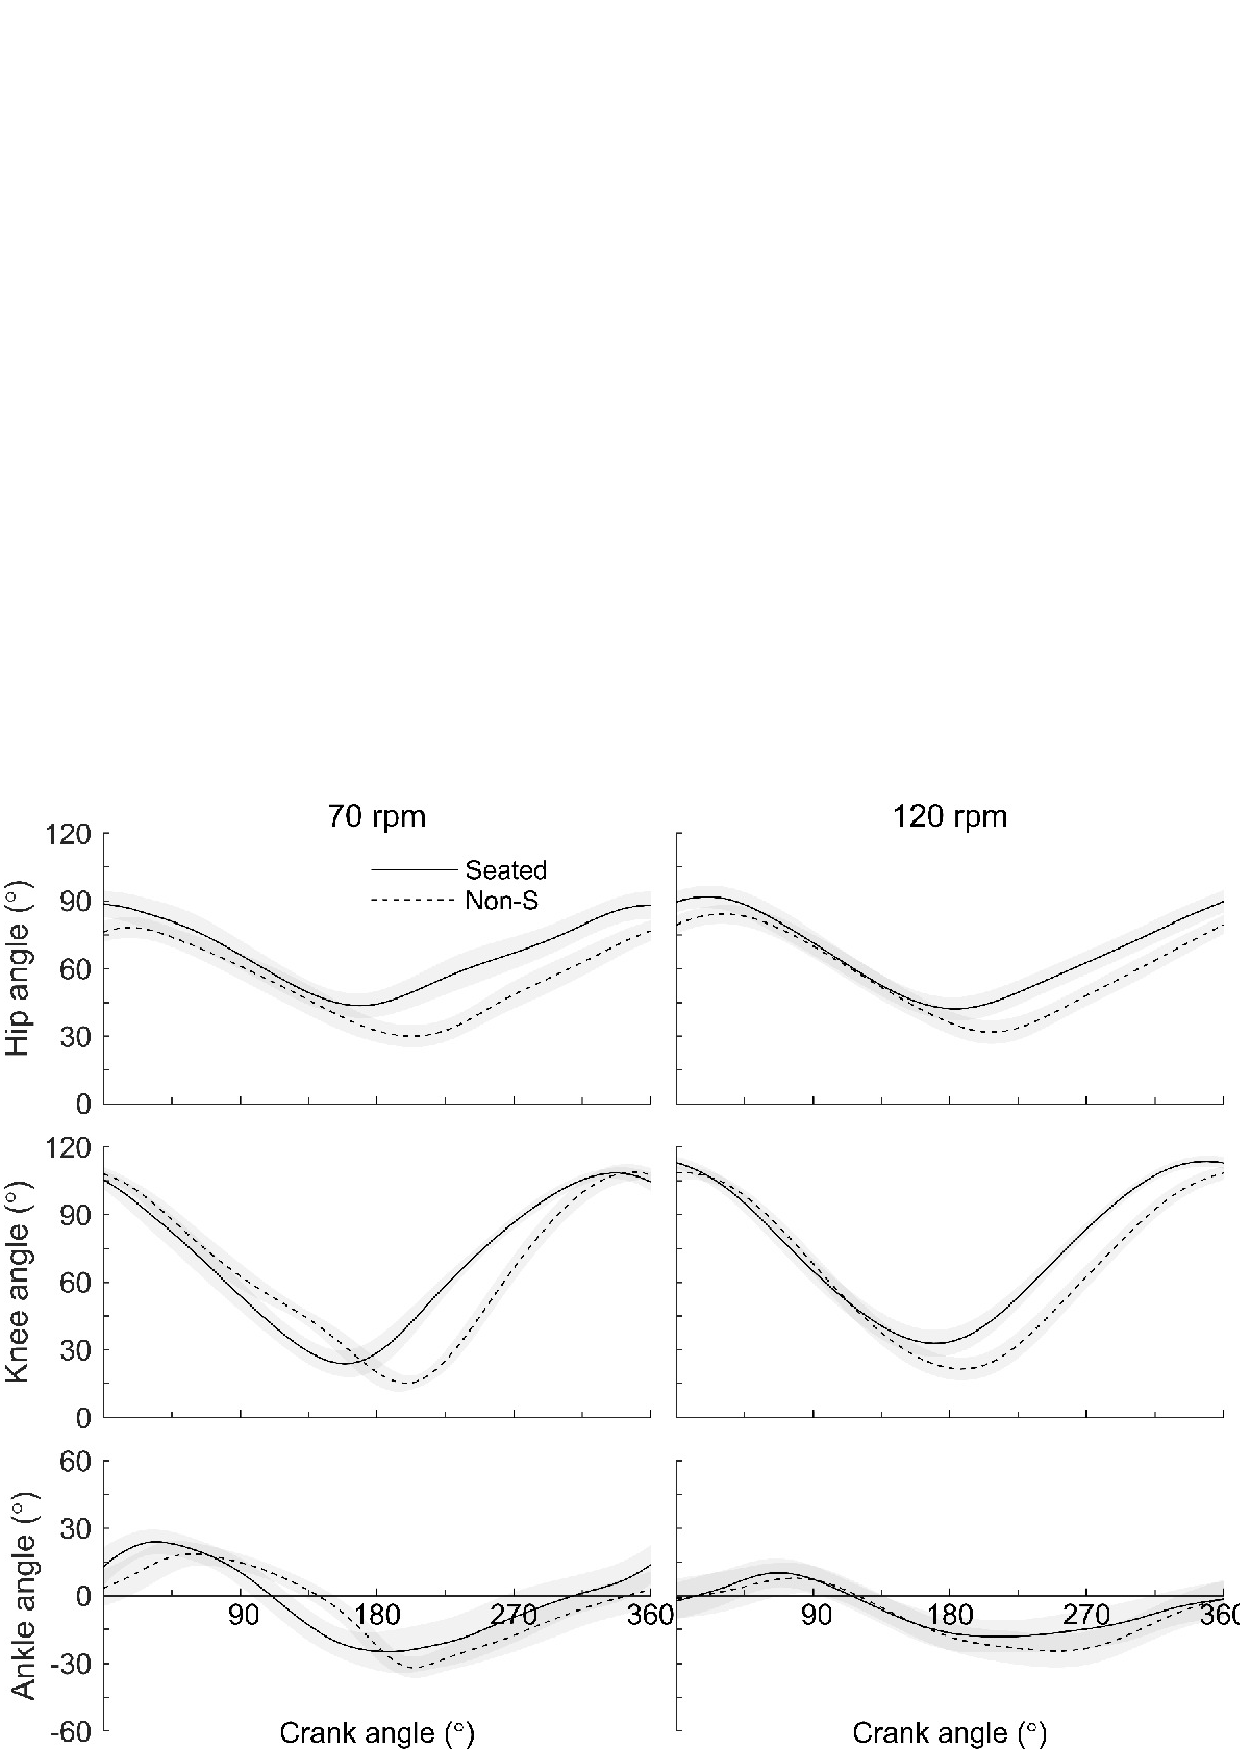
\includegraphics[width=\textwidth]{SupplementaryFigures/Study1_supp3.png}
    \caption[The hip, knee, and ankle extend later in the crank cycle and to a greater extent when non-seated compared to when seated.]{\textbf{The hip, knee, and ankle extend later in the crank cycle and to a greater extent when non-seated compared to when seated.} Group mean ($\pm$SD, shaded area) joint angle with respect to crank angle at the hip, knee and ankle during each condition.}
    \label{fig:m1sdc3}
\end{figure}

\begin{figure}
    \centering
    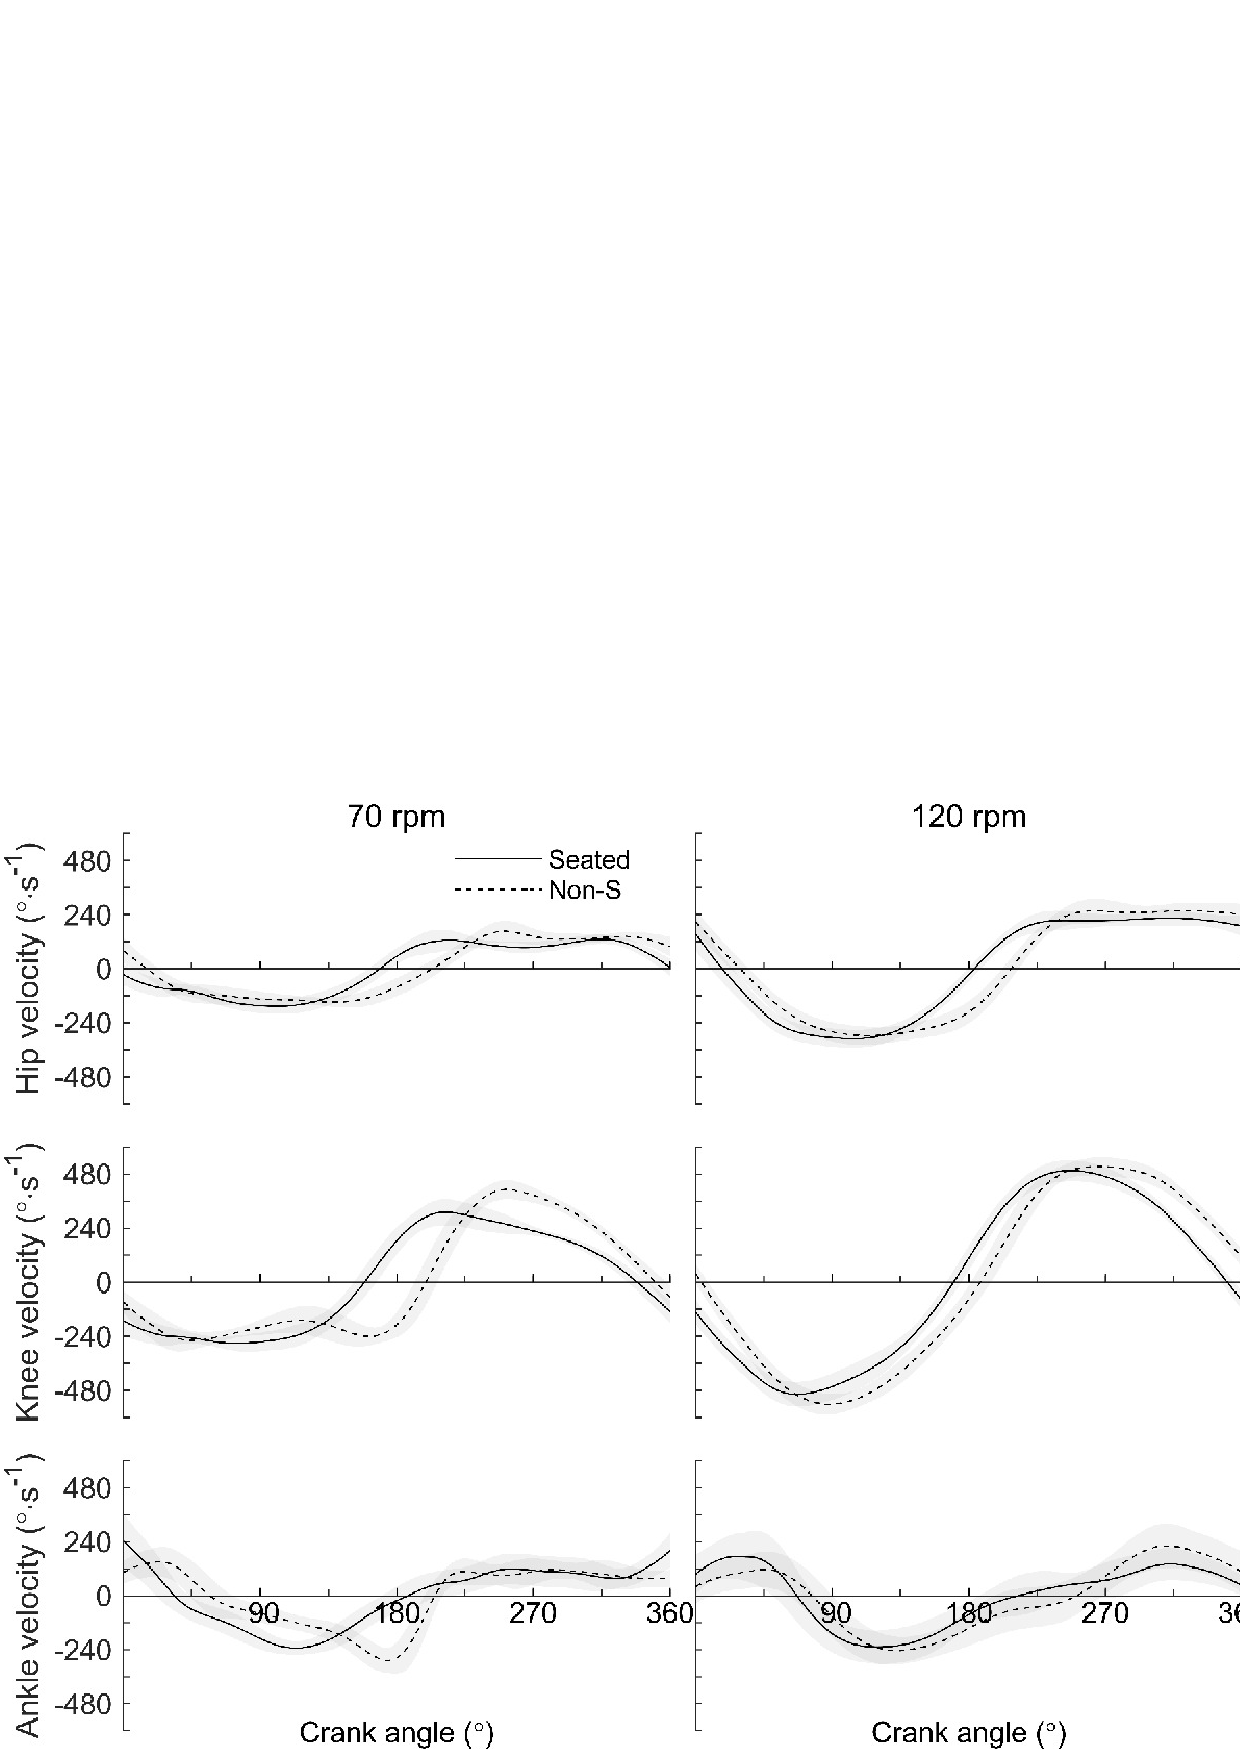
\includegraphics[width=\textwidth]{SupplementaryFigures/Study1_supp4.png}
    \caption[Duty cycle of the knee increased at 70 rpm when non-seated compared to when seated, which also resulted in greater peak knee flexion velocity.]{\textbf{Duty cycle of the knee increased at 70 rpm when non-seated compared to when seated, which also resulted in greater peak knee flexion velocity.} Group mean ($\pm$SD, shaded area) joint velocity with respect to crank angle at the hip, knee and ankle during each condition.}
    \label{fig:m1sdc4}
\end{figure}

\begin{figure}
    \centering
    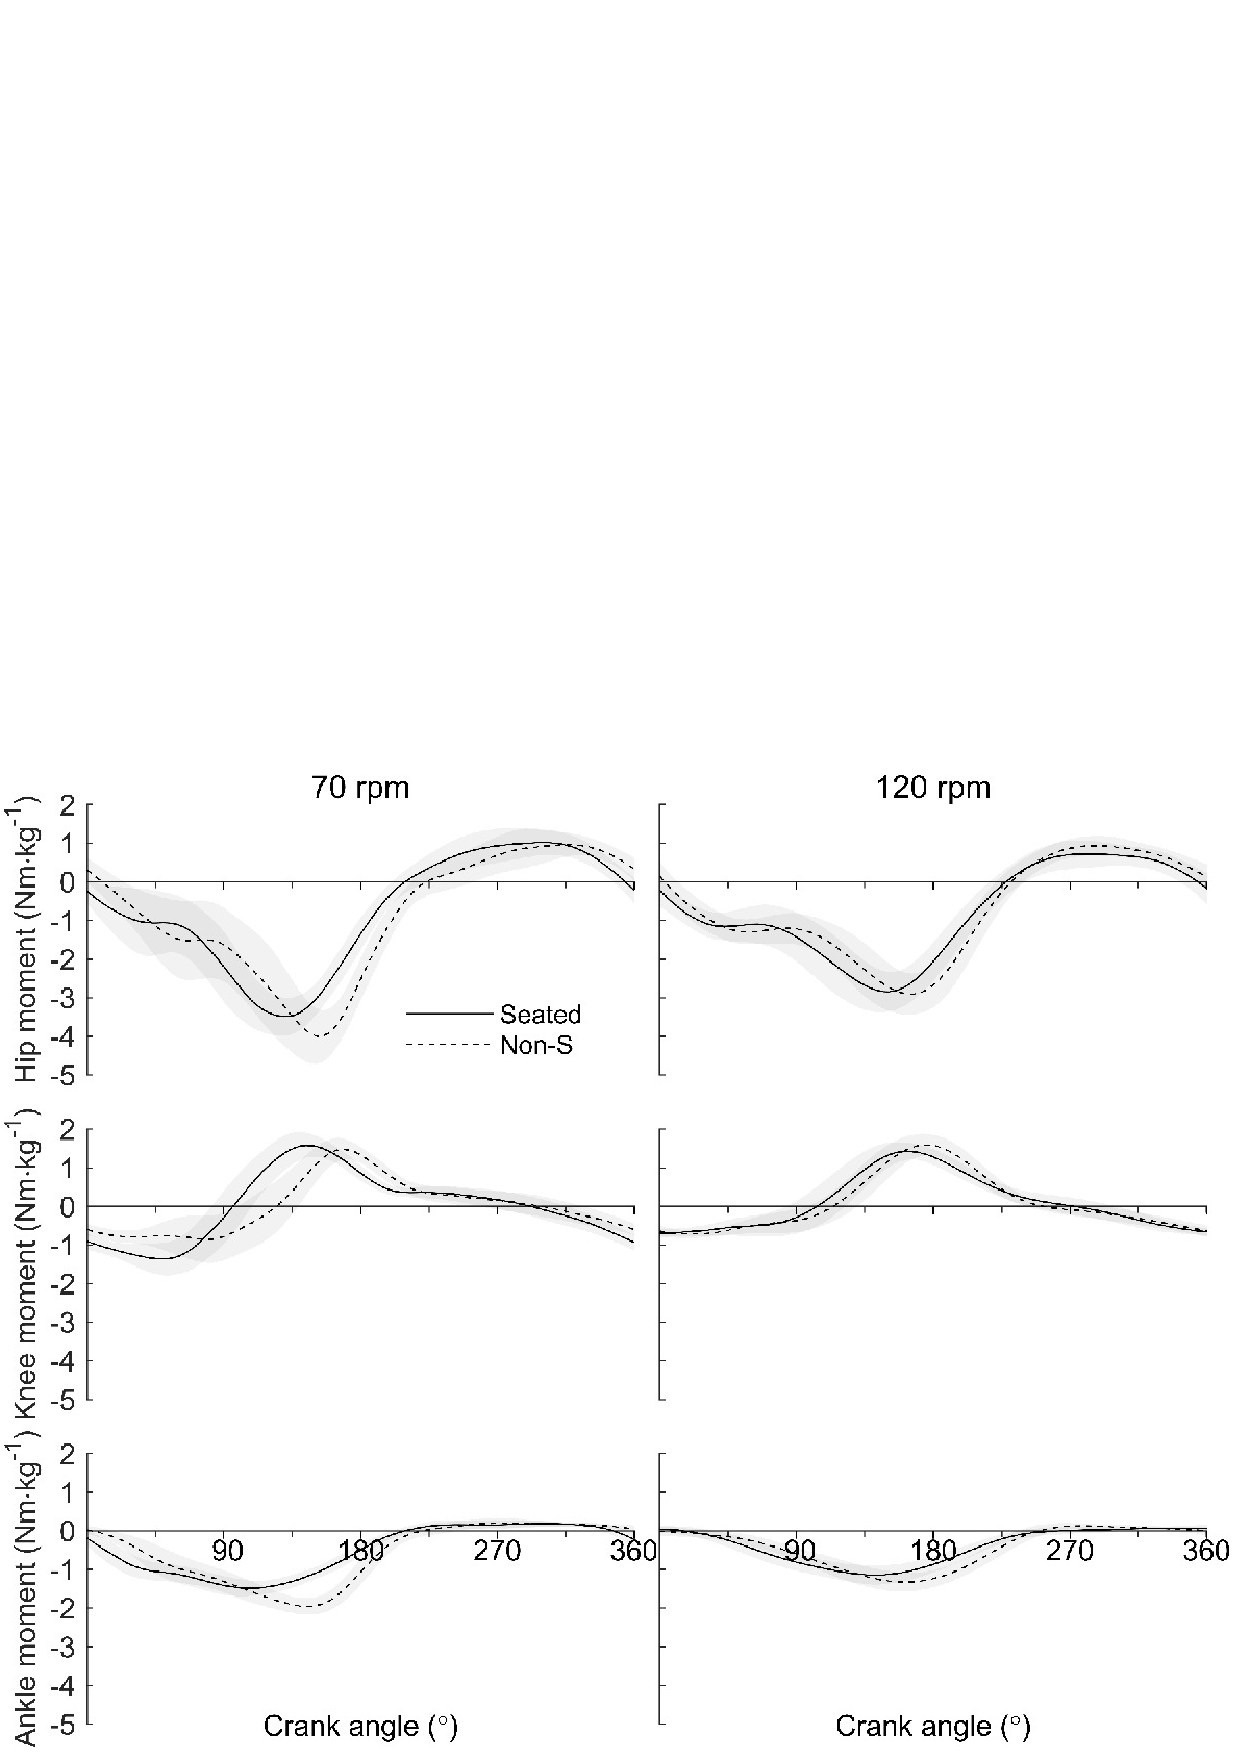
\includegraphics[width=\textwidth]{SupplementaryFigures/Study1_supp5.png}
    \caption[Peak hip extension moments and ankle plantar flexion moments increased when non-seated at 70 rpm, likely due to an increased redistribution of net joint moments by bi-articular muscles.]{\textbf{Peak hip extension moments and ankle plantar flexion moments increased when non-seated at 70 rpm, likely due to an increased redistribution of net joint moments by bi-articular muscles.} Group mean ($\pm$SD, shaded area) net joint moments with respect to crank angle at the hip, knee and ankle during each condition.}
    \label{fig:m1sdc5}
\end{figure}

\begin{figure}
    \centering
    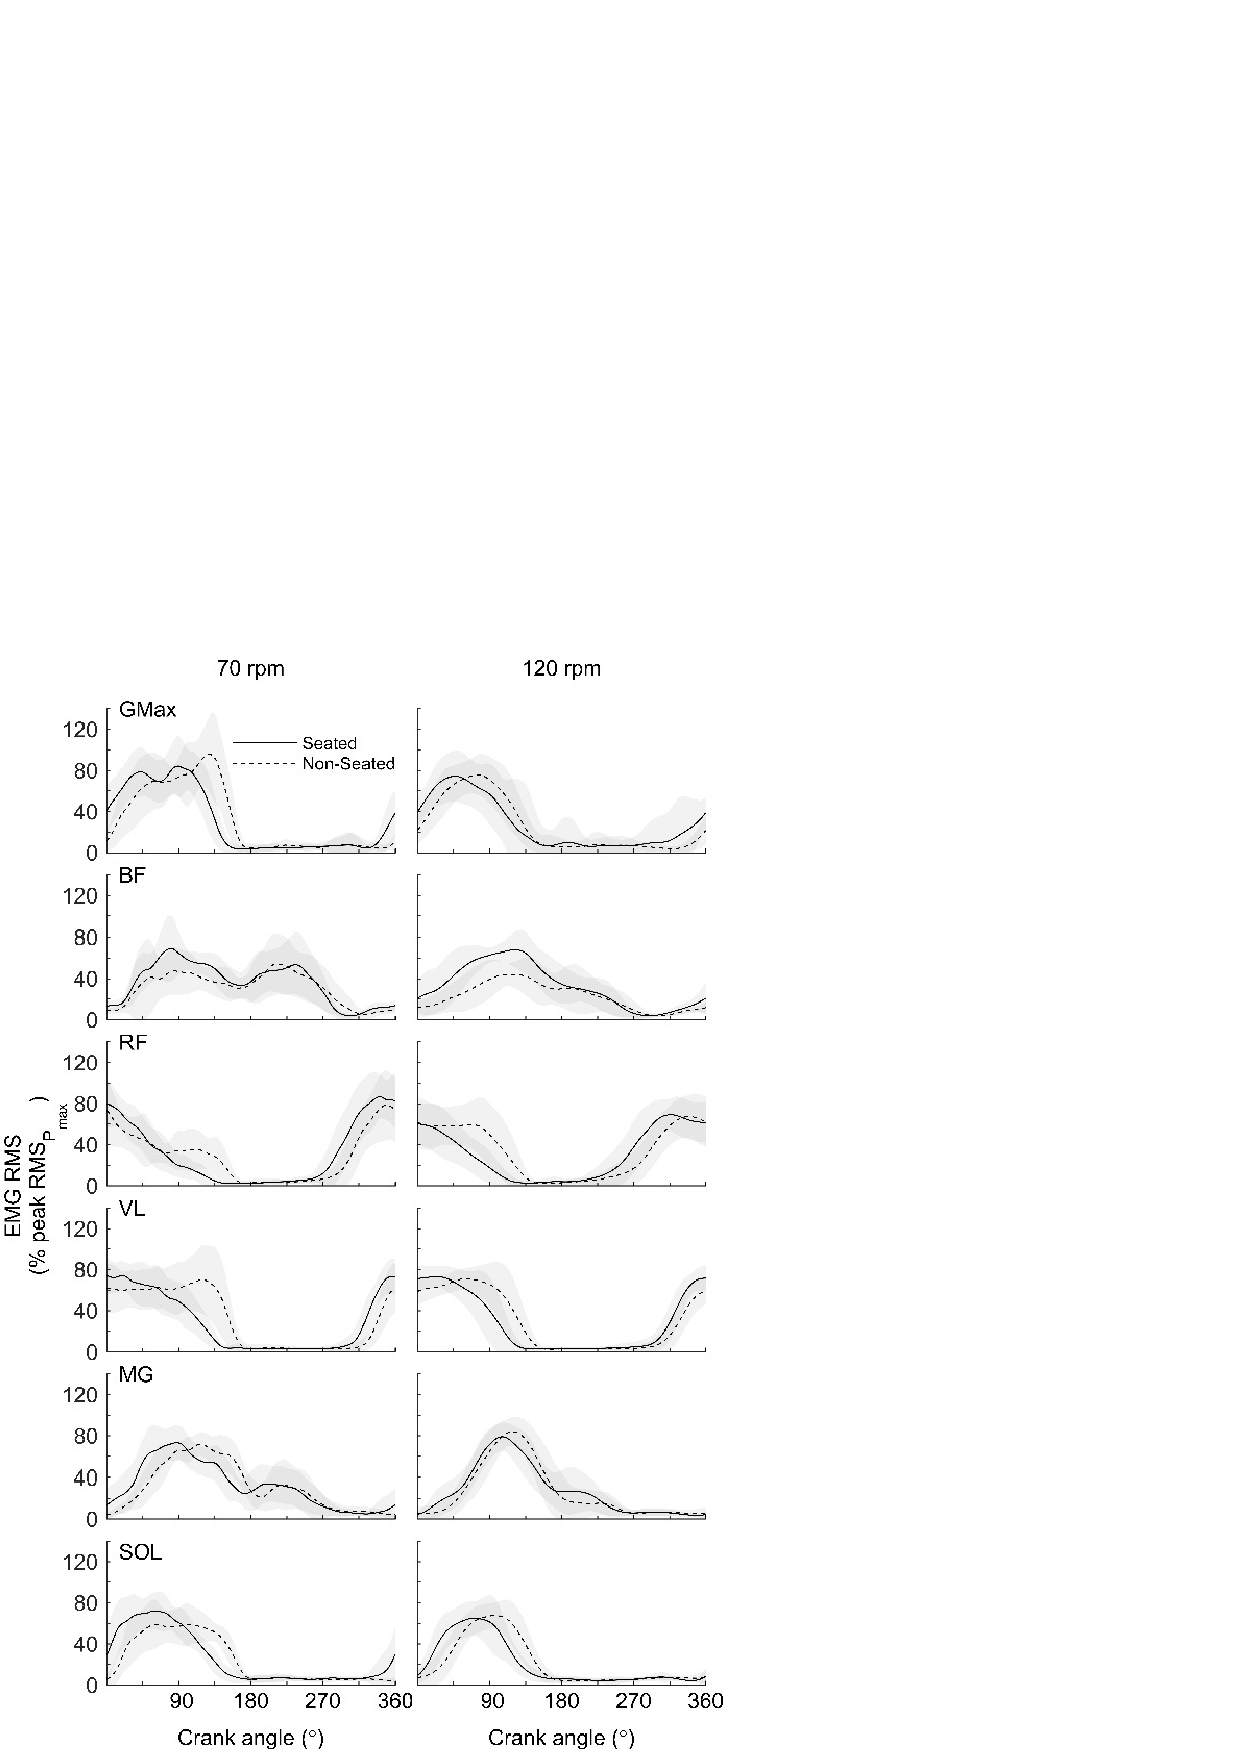
\includegraphics[width=0.85\textwidth]{SupplementaryFigures/Study1_supp6.png}
    \caption[The period of EMG activity of most muscles within the lower limb was shifted later in the crank cycle when cycling in a non-seated posture.]{\textbf{The period of EMG activity of most muscles within the lower limb was shifted later in the crank cycle when cycling in a non-seated posture.} Group mean ($\pm$SD, shaded area) EMG activity of muscles within the right lower limb with respect to crank angle during high-power output cycling at 70 rpm and 120 rpm in a seated and non-seated posture.}
    \label{fig:m1sdc6}
\end{figure}
\FloatBarrier

\section{Supplementary figure for study in Chapter 4}
\begin{figure}[htbp]
    \centering
    \includegraphics[width=\textwidth]{SupplementaryFigures/Study2_supp1.png}
    \caption[Rider CoM displacement occurred predominantly in the vertical direction during non-seated cycling.]{\textbf{Rider CoM displacement occurred predominantly in the vertical direction during non-seated cycling.} Data in the cubes show the group mean CoM trajectory (green) projected onto  three planes (black) during non-seated cycling under different power outputs (10$\%$, 30$\%$, and 50$\%$ P$_{max.i}$) at 70 rpm (left) and 120 rpm (right). The X, Y, and Z axes relate to CoM movement in the anterior-posterior, medio-lateral and vertical directions, respectively. Cartesian plots show the group mean CoM vertical displacement, velocity and acceleration with respect to crank angle (0\textdegree; top dead centre) under the same conditions. Note that displacement is the result of work done on, or by, the CoM. Velocity is the result of power generated on, or by, the CoM. Acceleration is the result of vertical interaction force between the bicycle and the rider.}
    \label{fig:m2f2}
\end{figure}
\FloatBarrier
\clearpage

\section{Supplementary figures for study in Chapter 5}
\begin{sidewaysfigure}[htbp]
    \centering
    \includegraphics[width=0.9\textwidth]{SupplementaryFigures/Study3_supp1.png}
    \caption[Riders appeared to dissipate power at the knee much earlier in the crank cycle when self-restricting bicycle lean.]{\textbf{Riders appeared to dissipate power at the knee much earlier in the crank cycle when self-restricting bicycle lean.} Group mean net joint moments, joint velocities, and joint power at the hip, knee, ankle in each condition. The altered pattern of power generation and dissipation within the right lower limb in the self-restricted condition points toward a greater demand on bi-articular knee extensors and flexors to transfer power from the knee to hip and ankle during the downstroke.}
    \label{fig:m3_sdc1}    
\end{sidewaysfigure}

\begin{sidewaysfigure}[htbp]
    \centering
    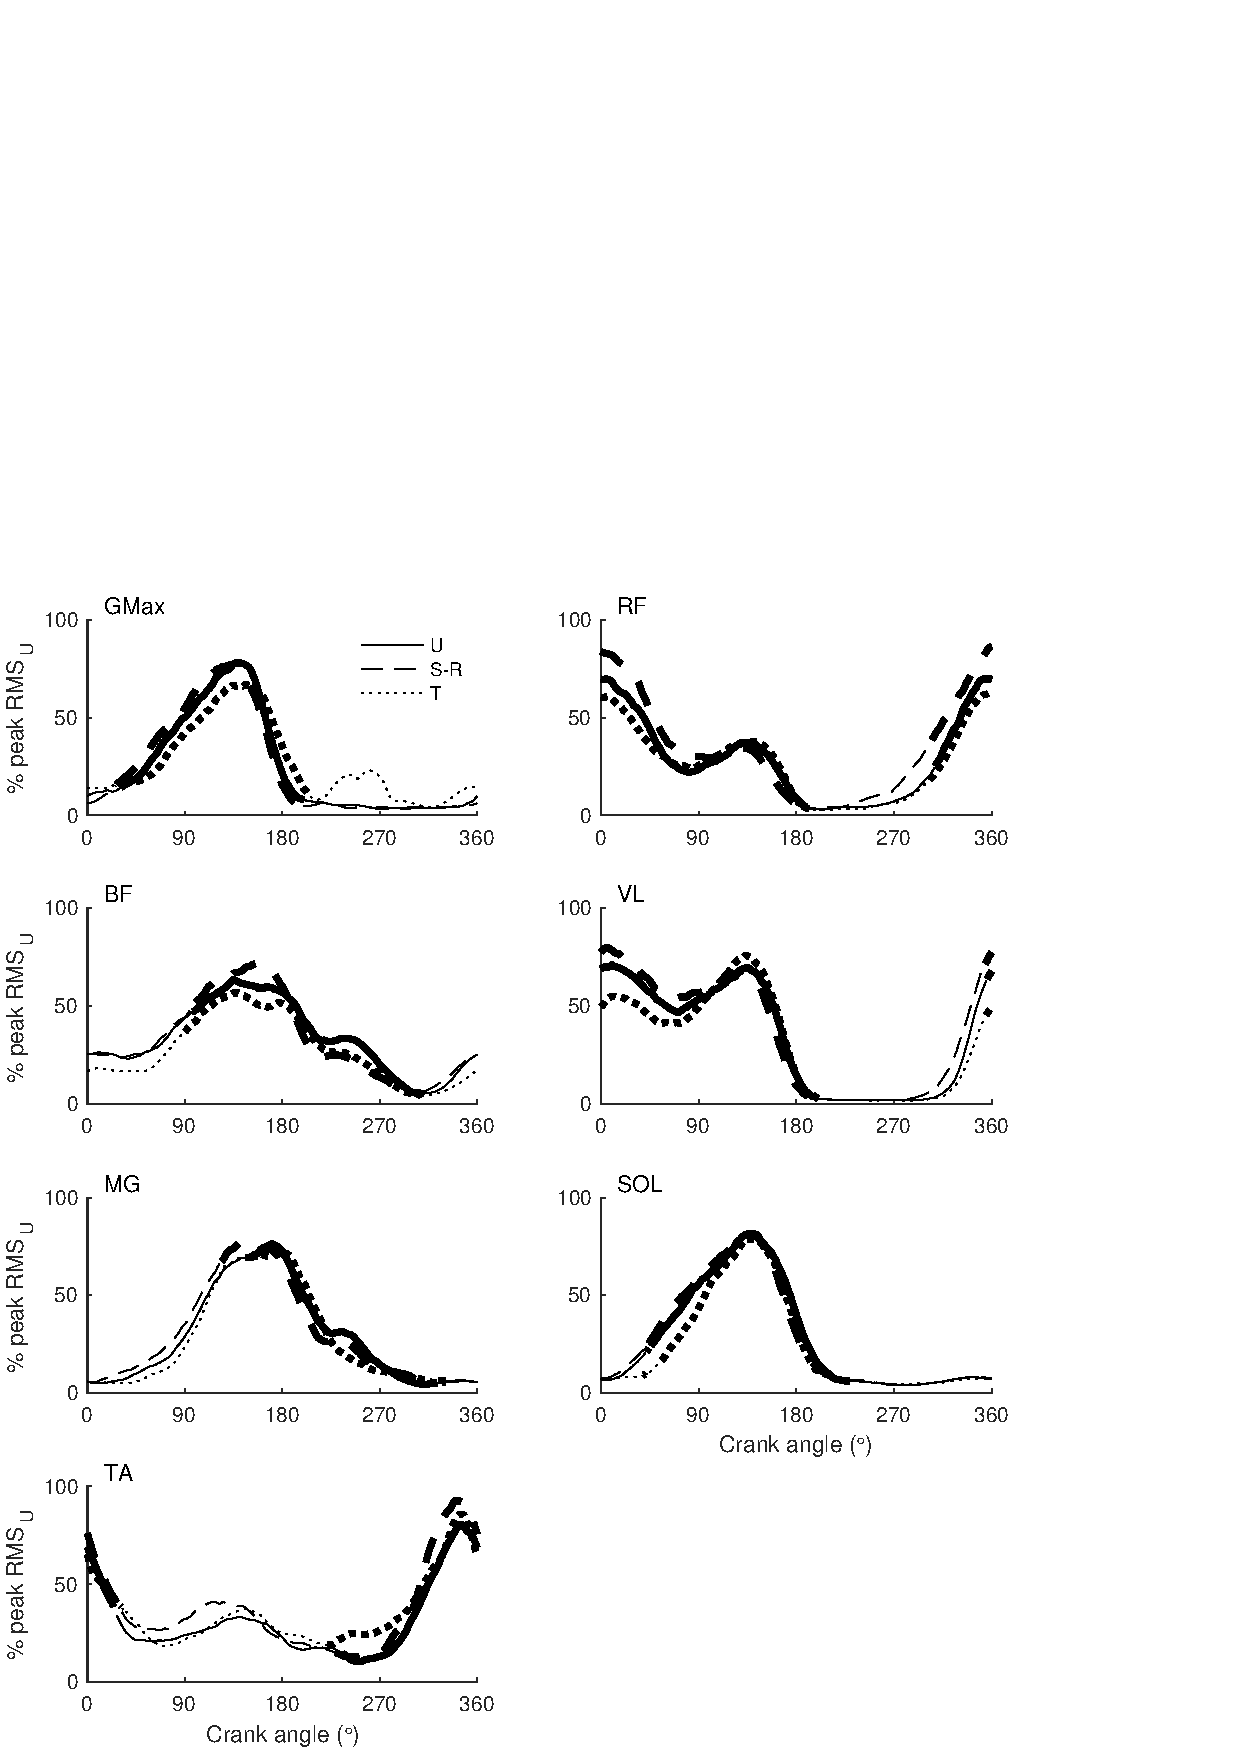
\includegraphics[width=0.9\textwidth]{SupplementaryFigures/Study3_supp2.pdf}
    \caption[Technical drawing of instrumented cranks used for study in Chapter \ref{Chap:5}.]{\textbf{Technical drawing of instrumented cranks used for study in Chapter \ref{Chap:5}.}} \label{fig:m3_sdc2}
\end{sidewaysfigure}
